\chapter{AwesomeChapterName}

\begin{itemize}
    \item canonical = constant $N$, $V$ and $T$
    \item microcanonical = constant $N$, $V$ and $E$
\end{itemize}


\section{Ensemble/thermostats}
We have now developed a molecular dynamics program that simulates simple systems \hl{like liquid/gas Argon}, with constant number of particles $N$, constant volume $V$ and constant energy $E$ \hl{$V$ and $E$ depend on integrator?}, which means that the system can't exchange particles or energy with the environment. This forms a statistical ensemble called the microcanonical ensemble or the $NVE$-ensemble, \hl{which has some implications for what we can measure?}. Other ensembles that might be of interest \hl{is/are?} the canonical ensemble (constant $N$, $V$ and temperature $T$) and the grand canonical ensemble (constant chemical potential $\mu$, $V$ and $T$) \hl{and $NPT$? see Thijssen p. 209(222)}.

\hl{To study the canonical ensemble we can use a thermostat, which is a method for controlling the temperature of the system.} \todo{transition to parts below}

The most often studied ensemble other than the microcanonical is the canonical, with constant temperature instead of energy. To study this we need a way of controlling the temperature of the system, which is usually done by using a \emph{thermostat}. A thermostat simulates the system being in contact with a heat bath with temperature $T_\text{bath}$. \todo{small discussion of how heat bath really works? see thijssen p. 203(216)} We measure the temperature via the kinetic energy of the system, so we know we have to \hl{modify} the velocities of the system to control the temperature. 

\orangebox{
    \begin{itemize}
        \item Thermostats == change ensemble
        \item Measure pressure, Frenkel eq. (3.4.1) p. 52.
        \item Measure temperature, Frenkel eq. (4.1.1) and (4.1.2) p. 64
    \end{itemize}
}

\subsection{Berendsen thermostat}
Perhaps the simplest example of a thermostat is the Berendsen thermostat\cite{berendsen1984molecular}, which \hl{simply} rescales all velocities by muliplying them with a factor $\gamma$
\begin{align*}
    \gamma = \sqrt{1 + \frac{\Delta t}{\tau}\left(\frac{T_\text{bath}}{T} - 1\right)},
\end{align*}
where $\Delta t$ is the timestep used in the simulations, $\tau$ controls the \hl{strength} of the thermostat (setting $\tau = \Delta t$ makes the temperature \hl{exactly constant equal to $T_\text{bath}$}), $T$ is the temperature of the system and $T_\text{bath}$ is the temperature of the \hl{simulated} heat bath. The velocities should be multiplied by this factor every timestep \hl{after calculating the new velocities}. An example of how to apply the Berendsen thermostat can be seen in \cref{list:applyBerendsenThermostat}.
%
\begin{listing}[!htb]%
\begin{cppcode*}{gobble=4}
    void applyBerendsenThermostat(System &system, double T, double Tbath, 
        double dt, double tau)
    void applyBerendsenThermostat(vector<Atom*> &atoms, double T, double Tbath, 
        double dt, double tau)
    {
        double gamma = sqrt(1 + dt/tau(Tbath/T - 1));
        for (Atom *atom : system.atoms())
        for (Atom *atom : atoms)
        {
            atom->velocity() *= gamma;
        }
    }
\end{cppcode*}
\caption{%
    \texttt{applyBerendsenThermostat}. \hl{decide on System or vector<Atom*> as input}%
    \label{list:applyBerendsenThermostat}%
}%
\end{listing}%

\subsection{Nos\'e-Hoover}
\orangebox{
    \begin{itemize}
        \item Nosé-Hoover and Nosé-Hoover chains
    \end{itemize}
}



\section{Observables? Measurements?}
% To measure an observable quantity in a simulation we must be able to express it as a function of the positions, velocities and forces on the particles in the system. 
% 
% According to the equipartition principle, the average total kinetic energy $\langle E_k \rangle$ is
% \begin{align*}
%     \left\langle E_k \right\rangle = \left\langle \frac{1}{2}mv^2 \right\rangle = \frac{3}{2}Nk_B T,
% \end{align*}
% from which we can derive the temperature of the system. Here $m$ is the mass of a particle, $v$ is the speed of a particle, and $T$ is the corresponding temperature of the system.
% 
% An often used method for measuring the pressure $P$ is derived from the virial equation for the pressure, which gives
% \begin{align*}
%     P = \rho k_B T + \frac{1}{3V}\sum_i \sum_{j>i} \bvec F(\rvec_{ij}) \cdot \rvec_{ij},
% \end{align*}
% where $V$ is the volume, $\rho$ is the atom density, $\bvec F(\bvec r)$ is the force between two atoms separated by $\bvec r$, and $\rvec_{ij} = \rvec_j - \rvec_i$ is the vector between atom $i$ and atom $j$. \hl{1) this equation depends on the ensemble, and is only valid for micro-canonical ensemble -- project 1 FYS4460} \hl{2) this expression is derived for a system at constant $N$, $V$, and $T$, see Frenkel p. 84(104) sec. 4.4}.
%
%
%
\begin{listing}[!htb]%
\begin{cppcode*}{gobble=4}
    void sample(System &system)
    {
    }
\end{cppcode*}
\caption{%
    \hl{FINISH THIS LISTING}. Implementation of the function \texttt{sample} from \cref{list:simple_md_program}.%
    \label{list:sampling}%
}%
\end{listing}%
\todo{finish this listing}


\subsection{Temperature}
According to the equipartition principle the average total kinetic energy \hl{per atom}, for a system consisting of $N$ particles with three degrees of freedom each, can be related to the temperature of the system via
\begin{align*}
    \Braket{E_k} = \frac{3}{2}Nk_\text{B}T,
\end{align*}
where $T$ is the temperature of the system. We calculate the average kinetic energy using
\begin{align*}
    \Braket{E_k} = \frac{1}{2N}\sum_{i=1}^N m_i v_i^2,
\end{align*}
where $m_i$ and $v_i = |\vec v_i|$ is respectively the mass and speed of atom $i$. 

See \cref{list:temperatureSample} for an example of how to calculate the temperature in a molecular dynamics simulation.
%
\begin{listing}[!htb]%
\begin{cppcode*}{gobble=4}
    double temperatureSample(System &system)
    {
        double kineticEnergy = 0.0;
        for (Atom *atom : system.atoms())
        {
            kineticEnergy += atom->velocity().lenghtSquared();
        }

        kineticEnergy *= 0.5;
        double temperature = 2.0*kineticEnergy/(3.0*system.nAtoms()
                                                *boltzmannConstant);  // SI units
        return temperature;
    }
\end{cppcode*}
\caption{%
    An example of how to calculate the temperature in a molecular dynamics simulation. Example implementation of \texttt{temperatureSample} from \cref{list:sampling}.%
    \label{list:temperatureSample}%
}%
\end{listing}%

\todo[inline]{Something about temperature in system with flow? (not that relevant for me though...)}

\subsection{Pressure}
To measure the pressure when using potentials with pairwise additive interactions, like the case is for our example program with the Lennard-Jones potential, we can use a method derived from the virial equation for the pressure\cite[Section~4.4]{frenkel2001understanding}. In a volume $V$ with particle density $\rho = N/V$, the average pressure is
% For pairwise additive interactions we can write\cite[Section~4.4]{frenkel2001understanding}
\begin{align}
    P = pk_\text{B}T + \frac{1}{dV} \Braket{\sum_{i<j} \bvec F (\bvec r_{ij}) \cdot \bvec r_{ij}},
    \label{eq:measure_pressure}
\end{align}
where $\vec F(\rvec_{ij})$ is the force between particle $i$ and $j$, and $\rvec_{ij}$ is the distance between the particles. \hl{Note that this expression for the pressure has been derived for a system at constant $N$, $V$ and $T$, whereas our simulations are performed at a constant $N$, $V$, and $E$}

We see that we need the force from each atom $j$ on atom $i$, $\vec F(\rvec_{ij})$ to calculate the pressure, so for efficiency we should calculate the contribution to the pressure, $\vec F(\rvecij)\cdot\rvecij$, while doing the force calculations. The contribution to the pressure should then be stored so we can calculate the average in \cref{eq:measure_pressure} later.

An example of how to calculate the pressure in a molecular dynamics simulation can be seen in \cref{list:pressureSample}.
%
\begin{listing}[!htb]%
\begin{cppcode*}{gobble=4}
    double pressureSample(System &system, double temperature)
    {
        double pressure;
        for (Atom *atom : system.atoms())
        {
            pressure += atom->pressure();
        }
        pressure /= (3.0*system.volume());
        double density = system.nAtoms()/system.volume(); // Assume homogeneous
        pressure += density*boltzmannConstant*temperature; // SI units
        return pressure;
    }
\end{cppcode*}
\caption{%
    An example of how to calculate the pressure in a molecular dynamics simulation. Example implementation of \texttt{pressureSample} from \cref{list:sampling}. Not that this function needs the temperature of the system as input, and assumes that the system is homogeneous, so we can estimate the density using $\rho = N/V$. We assume that the contribution to the pressure from each atom $\sum_{i<j}\vec F(\rvec_{ij})\cdot\rvec_{ij}$ (stored as \texttt{atom->pressure()}) has been calculated previously. This is usually calculated while calculating the forces between the atoms, since we need $\vec F(\rvec_{ij})$.%
    \label{list:pressureSample}%
}%
\end{listing}%

\subsection{Diffusion}
We can measure the diffusion constant $D$ by measuring the square displacement $r_i^2(t)$ of each atom as a function of time, and averaging over all atoms. We measure the mean square displacement as
\begin{align*}
    \Braket{r^2(t)} = \frac{1}{N} \sum_{i=1}^N \left( \rvec_i(t) - \rvec_i(t=0) \right)^2,
\end{align*}
where $\rvec_i(t=0)$ is the initial position of atom $i$. From theoretical considerations of the diffusion process we can relate the diffusion constant to the mean square displacement through\cite[Section~4.4.1]{frenkel2001understanding}
\begin{align*}
    &\Braket{r^2(t)} = 2dDt &\text{when }t\rightarrow \infty,
\end{align*}
where $d$ is the \hl{spatial} dimensionality. This means that we can find the diffusion constant in a molecular dynamics simulation by measuring the mean square displacement for many timesteps, and plotting $\Braket{r^2(t)}/(2dt)$ as a function of time. The diffusion constant will then be the value this expression approaches when simulating for enough timesteps.

An example of how to measure the mean square displacement in a molecular dynamics simulation can be seen in \cref{list:diffusionSample}.
% Fick's law relates flux $\bvec j$ of diffusing species to the concentration gradient $\bvec \nabla c$ of the species
% \begin{align*}
%     \bvec j = -D\bvec \nabla c,
% \end{align*}
% where $D$ is the proportionality constant called the diffusion \hl{coefficient/constant}.
% 
% Conservation of \hl{species/atoms?}
% \begin{align*}
%     \dpd{c(r,t)}{t} + \div \cdot \vec j(r,t) = 0,
% \end{align*}
% which gives
% \begin{align}
%     \dpd{c(r,t)}{t} - D\nabla^2 c(r,t) = 0.
%     \label{eq:diffusion_diff}
% \end{align}
% % We can solve this equation with the boundary condition
% % \begin{align*}
% %     c(r,0) = \delta (r),
% % \end{align*}
% % where $\delta(r)$ is the Dirac delta function, which gives
% % \begin{align*}
% %     c(r,t) = \frac{1}{(4\pi Dt)^{d/2}} \exp\left(-\frac{r^2}{4Dt}\right).
% % \end{align*}
% By multiplying \cref{eq:diffusion_diff} by $r^2$ and integrating over all space we get
% \begin{align*}
%     \dpd{}{t}\int \drvec~ r^2 c(r,t) = D\int \drvec~ r^2 \nabla^2 c(r,t).
% \end{align*}
% We recognize the integral on the left-hand side as the the mean square displacement %\hl{time dependence of the second moment of $c(r,t)$???}
% \todo{what???}
% \begin{align*}
%     \int \drvec~ c(r,t) r^2 \equiv \Braket{r^2(t)},
% \end{align*}
% where we have imposed
% \begin{align*}
%     \int \drvec~ c(r,t) = 1.
% \end{align*}
% Applying partial integration to the right-hand side we obtain
% \begin{align*}
%     \dpd{\Braket{r^2(t)}}{t} 
%     &= D\int \drvec~ r^2 \nabla^2 c(r,t) \\
%     &= D\int \drvec~ \div \cdot \left(r^2\nabla c(r,t)\right) - D\int\drvec~ \div r^2 \cdot \nabla c(r,t) \\
%     &= D\int \dif \vec S~ \left(r^2\div c(r,t)\right) - 2D\int\drvec~ \rvec \cdot\div c(r,t) \\
%     &= 0 - 2D\int\drvec~ (\div \cdot \rvec c(r,t)) + 2D\int\drvec~ (\div \cdot \rvec) c(r,t) \\
%     &= 0 + 2dD\int \drvec~ c(r,t) \\
%     &= 2dD
% \end{align*}
% 
% 
% \begin{align*}
%     \dpd{\Braket{r^2(t)}}{t} = 6D
% \end{align*}
% $\Rightarrow$ Plot mean square distance as function of time
% \begin{align*}
%     \Braket{\delta r(t)^2} = \frac{1}{N} \sum_{i=1}^N \delta \rvec_i(t)^2
% \end{align*}
% and find $6D$ as slope of plot \hl{(after a while?)}
%
\begin{listing}[!htb]%
\begin{cppcode*}{gobble=4}
    double diffusionSample(System &system)
    {
        double rSquared = 0.0;
        for (Atom *atom : system.atoms())
        {
            drVec = atom->positiom() - atom->initialPosition() 
                    + atom->getBoundaryCrossings()*system.size();
            rSquared += drVec.lengthSquared();
        }
        rSquared /= system.nAtoms();
        return rSquared;
    }
\end{cppcode*}
\caption{%
    An example of how to calculate the mean square displacement in a molecular dynamics simulation. Example implementation of \texttt{diffusionSample} from \cref{list:sampling}. We store the inital positions of the atoms as \texttt{atom->initialPosition()}, and when using periodic boundary conditions we count the number of times we have to translate the atom one system-size in each direction, so while the position of the atom will always be inside the system, the \hl{\emph{real}} position of the atom can be calculated by adding \texttt{atom->getBoundaryCrossings()*system.size()} to $\rvec$.%
    \label{list:diffusionSample}%
}%
\end{listing}%


















\chapter{ChapterName}
\section{(Initialization) A typical experimental procedure}
When doing \hl{``experiments''} using molecular dynamics we use a procedure \hl{akin to/mimicing} that used by \hl{actual} experiments. Since the duration of the experiments we are realistically able to simulate on are of the order $10^{-9} s$ / nanoseconds or below, we have to be smart when initializing the system, to avoid having to simulate for a long time to get to the state we want to study. This means that we should start out with the system in a configuration/state as close to the one we want to study as possible. The problem with this when simulating \hl{silica/glass} is that the silica structure formed when rapidly cooling molten silica doesn't have any long-range ordering. Silica in the glass form has an amorph structure, which doesn't have any long-range ordering, but has short-range ordering ``well beyond the Si-O bond length''. This structure is hard to set up with an algorithm.

\orangebox{}{
    \begin{itemize}
        \item Remove drift!
        \item Something smart about why the small timescales doesn't matter that much, since the length scales are equally small?
        \item Short/long-range order
        \item Glass transition temperature
    \end{itemize}
    \begin{quote}
        ``
        When molten silicon dioxide SiO2 is rapidly cooled, it does not crystallize but solidifies as a glass. The geometry of the silicon and oxygen centers in glass is similar to that in quartz and most other crystalline forms of the same composition, i.e., silicon is surrounded by a regular tetrahedra of oxygen centers. The difference between the glass and the crystalline forms arise from the connectivity of these tetrahedral units. Although there is no long range periodicity in the glassy network there remains significant ordering at length scales well beyond the SiO bond length. One example of this ordering is found in the preference of the network to form rings of 6-tetrahedra.[18]
        
        The glass transition temperature of pure SiO2 is about 1475 K.
        ''
        
        \url{http://en.wikipedia.org/wiki/Silicon_dioxide#Fused_quartz}
    \end{quote}
}

To generate silica in the glass form we first create a perfect silica crystal in the crystalline form $\upbeta$-cristobalite, as see in figure \cref{fig:cristobalite} \todo{Why?}, and give the atoms a random uniformly distributed velocities with mean $\mu = 0$ and standard deviation $\sigma = \sqrt{T}$, where $T$ is the wanted temperature \hl{in MD units}. The crystal consists of corner-bonded SiO$_4$ tetrahedra, and in the perfect crystallic form all silicon atoms are bound to four oxygen atoms, and all oxygen atoms to two silicon atoms.
%
\begin{figure}[htpb]%
    \centering%
    \begin{subfigure}[c]{0.25\textwidth}%
%         \begin{minipage}[c]{\textwidth}%
        \includesvg[width=\textwidth, svgpath=./images/beta_cristobalite/]{beta_cristobalite_x01}%
%         \end{minipage}%
%         \caption{\cite{wikiCristobalite01}}%
        \caption{}%
        \label{fig:cristobalite01}%
    \end{subfigure}%
    \hspace{0.07\textwidth}%
    \begin{subfigure}[c]{0.45\textwidth}%
%         \begin{minipage}[c]{\textwidth}%
        \includesvg[width=\textwidth, svgpath=./images/beta_cristobalite/]{beta_cristobalite_xyz01}%
%         \end{minipage}%
%         \caption{\cite{wikiCristobalite02}}%
    \caption{}%
    \label{fig:cristobalite02}%
    \end{subfigure}%
    \caption{%
        Illustrations of the $\upbeta$-cristobalite structure, from two different views. Images from Wikipedia Commons, released to the public domain\cite{wikiCristobalite01,wikiCristobalite02}.%
        \label{fig:cristobalite}%
    }%
\end{figure}%

We then heat the system to 4500 K in steps of 700 K to melt the silica crystal. We alternate between using a thermostat to adjust the temperature and simulating with the thermostat off to let the system thermalize. The number of timesteps we used for the thermostat period is around 2 500, and for the thermalization period around 10 000. We then cool the system by doing the previous procedure in reverse.

We now have a thermalized and \hl{(hopefully)} realistic silica crystal at near room temperature. From this crystal we cut out the fracture, passivate using one of the passivation methods, and fill the fracture with water molecules, \hl{and use steepest descent}. After filling the fracture with water we need to thermalize the system again, since the energy (and thereby the temperature) changes when we remove and insert atoms.

We are now ready to do measurements.

\section{Passivation}
Since we don't take into consideration molecular bonds in the silica when removing atoms to create pores, we get dangling unsaturated bonds in the system. We rectify this by passivating the system by inserting atoms on the dangling bonds, turning them into \hl{stable} silanol groups\todo{why silanol?}.

In the passivation procedure we do some basic assumptions, based on the chemical nature of silica and water. In the thermodynamically stable form, silica should have the following properties\todo{source?}:
\begin{itemize}
    \item Silicon atoms should have tetrahedral coordination, with four oxygen atoms surrounding each silicon atom in a tetrahedral \hl{shape}. \todo{On average, not all silica will have this. Something about bonds? bonded to four oxygen atoms?}
    \item Oxygen atoms should have two silicon \hl{neighbors}\todo{not all, on average}.
    \item The Si-O distance should be in the range 1.5-1.9 pm\todo{source?} (depending on the crystalline form).
\end{itemize}

\hl{When removing atoms to create pores we don't care about these properties, which leads us to the following cases}
\begin{itemize}
    \item Silicon atoms with less than four oxygen neighbors.
    \item Oxygen atoms with one missing silicon neighbor.
    \item Silicon and oxygen atoms with no neighbors.
    \item \hl{Silicon and oxygen atoms with too many neighbors?}
\end{itemize}

\hl{When inserting oxygen and hydrogen we must make sure to inject neutrally, meaning twice as much hydrogen as oxygen (H$_2$O)}

Silicon atoms with less than four oxygen atoms bound to them get ($4-n_\text{O}$) hydroxide (OH$^-$) groups attached to them, where $n_\text{O}$ is the numer of oxygen atoms bound to the silicon. Oxygen atoms with a missing silicon neighbor get a hydrogen attached. 
% \hl{(oxygen atoms with two missing neighbors are removed)}.
% Oxygen atoms with less than two silicon atoms get ($2-n_\text{Si}$) hydrogen atom attached, where $n_\text{Si}$ is the number of silicon atoms bound to the oxygen. 

When passivating a silicon atom with missing oxygen neighbors by \hl{simply} filling in the missing atoms to complete the SiO$_4$-tetrahedra. We then put one hydrogen atom on each new oxygen atom, to avoid dangling bonds on the inserted oxygen atoms.

When passivating a oxygen atom with a missing silicon neighbor, we put one hydrogen atom on the opposite side of the oxygen atom compared to the silicon atom.

All silicon and oxygen atoms with no neighbors we remove, since they aren't really part of the silica.

To find the number of \hl{neighbors/bonds/bonded atoms} for each silicon and oxygen atom, we create what we call \emph{neigbor lists}, which is a list of atoms within a chosen radius, for each atom.
%
\begin{figure}[htpb]%
    \centering%
    \begin{subfigure}[b]{0.24\textwidth}%
        \includegraphics[width=\textwidth]{images/passivation/tetrahedra01.png}%
        \caption{}%
%         \caption{Illustration of how to divide a convex hexahedron into five tetraheda.}%
%         \label{fig:hex_to_tetra}%
    \end{subfigure}%
%     \hspace{5mm}%
    \begin{subfigure}[b]{0.24\textwidth}%
        \includegraphics[width=\textwidth]{images/passivation/tetrahedra02.png}%
        \caption{}%
%         \caption{A random fracture made from two periodic heightmaps.}%
%         \label{fig:fracture_model}%
    \end{subfigure}%
%     \hspace{5mm}%
    \begin{subfigure}[b]{0.24\textwidth}%
        \includegraphics[width=\textwidth]{images/passivation/tetrahedra03.png}%
        \caption{}%
%         \caption{A random fracture made from two periodic heightmaps.}%
%         \label{fig:fracture_model}%
    \end{subfigure}%
%     \hspace{5mm}%
    \begin{subfigure}[b]{0.24\textwidth}%
        \includegraphics[width=\textwidth]{images/passivation/tetrahedra04.png}%
        \caption{}%
%         \caption{A random fracture made from two periodic heightmaps.}%
%         \label{fig:fracture_model}\caption{}%
    \end{subfigure}%
    \caption{\hl{Caption}}%
    \label{fig:passivation}%
\end{figure}%

\begin{itemize}
    \item Tetrahedra
    \item Neighbor lists -- see base\_code/passivate\_using\_tetrahedra/passivator.cpp near line 700
    \begin{itemize}
        \item Create list of atoms in each voxel
        \item Create neighbor lists for each atom by looping through neighbor voxels for each atoms
    \end{itemize}
    \item Count number of neighbors of different types -- find number of missing neighbors, Si - 4 Oxygen, Oxygen 2 Si
    \item Insert OH on Si with missing O neighbors, insert H on Oxygen with missing Si neighbors
    \begin{itemize}
        \item Insert O/H at good angles
    \end{itemize}
    \item Improvement: find the atoms near surface using voxels, only passivate those atoms
\end{itemize}

\section{Injecting water}
To fill the pore we have made \hl{(after passivating the system)} we use the technique of \emph{voxelation} (see \cref{sec:voxelation}), and put one water molecule in each unoccupied voxel. The water density is then controlled by the size of the voxels.

If we want to inject water with density $\rho$ [kg/m$^3$], we can find the voxel size we need using the molar mass of water, $M_\text{H$_2$O} = M = 0.0180158 \text{ kg/mol}$. We find the ``volume'' of a water atom in \Ang, the unit used in the \hl{MD integrator/program and output files}, as follows
\begin{align*}
    V 
    &= \frac{ M\text{ [kg/mol]} }{ \rho\text{ [kg/m$^3$]} } \\
    &= \frac{
            M\text{ [kg/mol]} \times \dfrac{1}{N_A \text{ [mol$^{-1}$]}}
        }{
            \rho\text{ [kg/m$^3$]} \times \left(10^{-10} \text{ [\AA/m]}\right)^3
        } \\
    &= \frac{M}{\rho} \times \frac{10^{-30}}{N_A} \text{ [\AA$^3$]},
%     \times \frac{N_A \text{ [mol$^{-1}$]}}{10^{-10} \text{ [\AA/m]}} 10 \text{ [m$^3$]} \\
\end{align*}
from which we find the size we need our voxels to be as
\begin{align*}
    L = \left(\frac{M}{\rho} \times \frac{10^{30}}{N_A}\right)^{1/3}\text{ [\AA]}.
\end{align*}

We then divide the system into voxels of length $L$. And put one water molecule with random orientation in the center of each empty voxel. The naive way of finding the empty voxels is to just find which voxel each existing silicon and oxygen atom is in, and mark those as occupied. But the amorph \hl{structure} of solid silica means that we have a lot of very small pores inside the matrix, which ends up as empty voxels. \todo{something about definition of a pore?}

What we do is to assign a radius to each atom type \todo{which is hard, Si-O, ???}, and mark all voxels with it's center within this radius as occupied.

\begin{itemize}
    \item Voxelize system -- size depends on wanted density
    \item Mark all voxels within distance from other atoms as occupied
    \item Fill other voxels with H2O with random O-H orientation, but correct angle
    \item Improvement: Use one voxel size in the beginning (to avoid one-voxel pores), and then use a smaller voxel size when injecting water
\end{itemize}

